\ifdefined\included
\else
\documentclass[a4paper,11pt,twoside]{StyleThese}
\usepackage{amsmath,amssymb, amsthm}             % AMS Math
\usepackage[T1]{fontenc}
\usepackage[utf8x]{inputenc}
\usepackage{babel}
\usepackage{datetime}

\usepackage{silence}

\WarningFilter{minitoc(hints)}{W0023}
\WarningFilter{minitoc(hints)}{W0028}
\WarningFilter{minitoc(hints)}{W0030}

\usepackage{lmodern}
\usepackage{tabularx}
%\usepackage{tabular}
\usepackage{multirow}
\usepackage{xspace}

\usepackage{hhline}
\usepackage[left=1.5in,right=1.3in,top=1.1in,bottom=1.1in,includefoot,includehead,headheight=13.6pt]{geometry}
\renewcommand{\baselinestretch}{1.05}

% Table of contents for each chapter

\usepackage[nottoc, notlof, notlot]{tocbibind}
\usepackage{minitoc}
\setcounter{minitocdepth}{2}
\mtcindent=15pt
% Use \minitoc where to put a table of contents

\usepackage{aecompl}

% Glossary / list of abbreviations

\usepackage[intoc]{nomencl}
\iftoggle{ThesisInEnglish}{%
\renewcommand{\nomname}{Glossary}
}{ %
\renewcommand{\nomname}{Liste des Abréviations}
}

\usepackage{etoolbox}
\renewcommand\nomgroup[1]{%
  \item[\bfseries
  \ifstrequal{#1}{A}{Number Sets}{%
  \ifstrequal{#1}{G}{Agents Beliefs and Action Models}{%
  \ifstrequal{#1}{N}{Navigation}{%
  \ifstrequal{#1}{O}{Ontology}{%
  \ifstrequal{#1}{R}{Referring Expression Generation}{%
  \ifstrequal{#1}{Z}{Controllable and Uncontrollable Agents Task Planning}{}}}}}}%
]}

\makenomenclature



% My pdf code

\usepackage{ifpdf}

\ifpdf
  \usepackage[pdftex]{graphicx}
  \DeclareGraphicsExtensions{.jpg}
  \usepackage[pagebackref,hyperindex=true]{hyperref}
  \usepackage{tikz}
  \usetikzlibrary{arrows,shapes,calc}
\else
  \usepackage{graphicx}
  \DeclareGraphicsExtensions{.ps,.eps}
  \usepackage[dvipdfm,pagebackref,hyperindex=true]{hyperref}
\fi

\graphicspath{{.}{images/}}

%% nicer backref links. NOTE: The flag ThesisInEnglish is used to define the
% language in the back references. Read more about it in These.tex

\iftoggle{ThesisInEnglish}{%
\renewcommand*{\backref}[1]{}
\renewcommand*{\backrefalt}[4]{%
\ifcase #1 %
(Not cited.)%
\or
(Cited in page~#2.)%
\else
(Cited in pages~#2.)%
\fi}
\renewcommand*{\backrefsep}{, }
\renewcommand*{\backreftwosep}{ and~}
\renewcommand*{\backreflastsep}{ and~}
}{%
\renewcommand*{\backref}[1]{}
\renewcommand*{\backrefalt}[4]{%
\ifcase #1 %
(Non cité.)%
\or
(Cité en page~#2.)%
\else
(Cité en pages~#2.)%
\fi}
\renewcommand*{\backrefsep}{, }
\renewcommand*{\backreftwosep}{ et~}
\renewcommand*{\backreflastsep}{ et~}
}

% Links in pdf
\usepackage{color}
\definecolor{linkcol}{rgb}{0,0,0.4} 
\definecolor{citecol}{rgb}{0.5,0,0} 
\definecolor{linkcol}{rgb}{0,0,0} 
\definecolor{citecol}{rgb}{0,0,0}
% Change this to change the informations included in the pdf file

\hypersetup
{
bookmarksopen=true,
pdftitle="Planning For Both Robot and Human: Anticipating and Accompanying Human Decisions",
pdfauthor="Guilhem BUISAN", %auteur du document
pdfsubject="Thèse", %sujet du document
%pdftoolbar=false, %barre d'outils non visible
pdfmenubar=true, %barre de menu visible
pdfhighlight=/O, %effet d'un clic sur un lien hypertexte
colorlinks=true, %couleurs sur les liens hypertextes
pdfpagemode=None, %aucun mode de page
pdfpagelayout=SinglePage, %ouverture en simple page
pdffitwindow=true, %pages ouvertes entierement dans toute la fenetre
linkcolor=linkcol, %couleur des liens hypertextes internes
citecolor=citecol, %couleur des liens pour les citations
urlcolor=linkcol %couleur des liens pour les url
}

% definitions.
% -------------------

\setcounter{secnumdepth}{3}
\setcounter{tocdepth}{2}

% Some useful commands and shortcut for maths:  partial derivative and stuff

\newcommand{\pd}[2]{\frac{\partial #1}{\partial #2}}
\def\abs{\operatorname{abs}}
\def\argmax{\operatornamewithlimits{arg\,max}}
\def\argmin{\operatornamewithlimits{arg\,min}}
\def\diag{\operatorname{Diag}}
\newcommand{\eqRef}[1]{(\ref{#1})}

\usepackage{rotating}                    % Sideways of figures & tables
%\usepackage{bibunits}
%\usepackage[sectionbib]{chapterbib}          % Cross-reference package (Natural BiB)
%\usepackage{natbib}                  % Put References at the end of each chapter
                                         % Do not put 'sectionbib' option here.
                                         % Sectionbib option in 'natbib' will do.
\usepackage{fancyhdr}                    % Fancy Header and Footer

% \usepackage{txfonts}                     % Public Times New Roman text & math font
  
%%% Fancy Header %%%%%%%%%%%%%%%%%%%%%%%%%%%%%%%%%%%%%%%%%%%%%%%%%%%%%%%%%%%%%%%%%%
% Fancy Header Style Options

\pagestyle{fancy}                       % Sets fancy header and footer
\fancyfoot{}                            % Delete current footer settings

%\renewcommand{\chaptermark}[1]{         % Lower Case Chapter marker style
%  \markboth{\chaptername\ \thechapter.\ #1}}{}} %

%\renewcommand{\sectionmark}[1]{         % Lower case Section marker style
%  \markright{\thesection.\ #1}}         %

\fancyhead[LE,RO]{\bfseries\thepage}    % Page number (boldface) in left on even
% pages and right on odd pages
\fancyhead[RE]{\bfseries\nouppercase{\leftmark}}      % Chapter in the right on even pages
\fancyhead[LO]{\bfseries\nouppercase{\rightmark}}     % Section in the left on odd pages

\let\headruleORIG\headrule
\renewcommand{\headrule}{\color{black} \headruleORIG}
\renewcommand{\headrulewidth}{1.0pt}
\usepackage{colortbl}
\arrayrulecolor{black}

\fancypagestyle{plain}{
  \fancyhead{}
  \fancyfoot{}
  \renewcommand{\headrulewidth}{0pt}
}

%\usepackage{MyAlgorithm}
%\usepackage[noend]{MyAlgorithmic}
\usepackage{algorithm}
\usepackage[noend]{algpseudocode}
\usepackage{comment}
\usepackage[ED=EDSYS-Robo, Ets=INSA]{tlsflyleaf}
%%% Clear Header %%%%%%%%%%%%%%%%%%%%%%%%%%%%%%%%%%%%%%%%%%%%%%%%%%%%%%%%%%%%%%%%%%
% Clear Header Style on the Last Empty Odd pages
\makeatletter

\def\cleardoublepage{\clearpage\if@twoside \ifodd\c@page\else%
  \hbox{}%
  \thispagestyle{empty}%              % Empty header styles
  \newpage%
  \if@twocolumn\hbox{}\newpage\fi\fi\fi}

\makeatother
 
%%%%%%%%%%%%%%%%%%%%%%%%%%%%%%%%%%%%%%%%%%%%%%%%%%%%%%%%%%%%%%%%%%%%%%%%%%%%%%% 
% Prints your review date and 'Draft Version' (From Josullvn, CS, CMU)
\newcommand{\reviewtimetoday}[2]{\special{!userdict begin
    /bop-hook{gsave 20 710 translate 45 rotate 0.8 setgray
      /Times-Roman findfont 12 scalefont setfont 0 0   moveto (#1) show
      0 -12 moveto (#2) show grestore}def end}}
% You can turn on or off this option.
% \reviewtimetoday{\today}{Draft Version}
%%%%%%%%%%%%%%%%%%%%%%%%%%%%%%%%%%%%%%%%%%%%%%%%%%%%%%%%%%%%%%%%%%%%%%%%%%%%%%% 

\newenvironment{maxime}[1]
{
\vspace*{0cm}
\hfill
\begin{minipage}{0.5\textwidth}%
%\rule[0.5ex]{\textwidth}{0.1mm}\\%
\hrulefill $\:$ {\bf #1}\\
%\vspace*{-0.25cm}
\it 
}%
{%

\hrulefill
\vspace*{0.5cm}%
\end{minipage}
}

\let\minitocORIG\minitoc
\renewcommand{\minitoc}{\minitocORIG \vspace{1.5em}}

\usepackage{multirow}
%\usepackage{slashbox}

\newenvironment{bulletList}%
{ \begin{list}%
	{$\bullet$}%
	{\setlength{\labelwidth}{25pt}%
	 \setlength{\leftmargin}{30pt}%
	 \setlength{\itemsep}{\parsep}}}%
{ \end{list} }

\theoremstyle{definition}
\newtheorem{definition}{Definition}
\renewcommand{\epsilon}{\varepsilon}

% centered page environment

\newenvironment{vcenterpage}
{\newpage\vspace*{\fill}\thispagestyle{empty}\renewcommand{\headrulewidth}{0pt}}
{\vspace*{\fill}}

\usepackage{tablefootnote}

\theoremstyle{plain}
\newtheorem{constraint}{Constraint}[section]

\algnewcommand\algorithmicforeach{\textbf{for each}}
\algnewcommand\algorithmicin{\textbf{in}}
\algdef{S}[FOR]{ForEach}[2]{\algorithmicforeach\ #1\ \algorithmicin\ #2\ \algorithmicdo}

\usepackage{listings}
\lstdefinestyle{customPlan}{
  language=C,
  commentstyle=\itshape\color{green!25!black},
}
\usepackage{pdfpages}

\sloppy
\begin{document}
\setcounter{chapter}{1} %% Numéro du chapitre précédent ;)
\dominitoc
\faketableofcontents
\fi

\chapter{Coplanning for navigation}
\minitoc

\section{Introduction}
In a lot of human robot interaction scenarios, the robot has to move in the environment to accomplish its task. It can either be that the task cannot be done in the direct vicinity of the robot or that the task itself is to move elsewhere. For example in the MuMMER project, a Pepper robot in a mall has to give direction instructions to guide a human to their wanted location. The robot is also able to point to visible landmarks to locate the beginning of the route (\textit{e.g.} saying \textit{"Take these stairs, then take the corridor on your right and the shop will be on your left" while pointing to the stairs}). However, some obstacles in the proximity of the robot and the guided human can prevent them to see the pointed landmarks, or a corridor crossing can be hidden, making the route description one step longer than it should be. Thus, to perform the task of route guiding more efficiently, the robot might decide to move.
In the Spencer project, another robot has to guide people to their gate in the Schipol airport. Here, the robot will navigate all the way from the starting point to the final destination while ensuring the human is actually following it, but also has to avoid other pedestrians. In this example, the navigation of the robot is a main part of the task.
In both example, the robot has to make plan its motion such as the physical and psychological safety of surrounding humans are ensured. However, not taking into account the motion of these humans during the planning process may lead to suboptimal trajectories or even deadlock.
We propose in this chapter to, after a survey of related works, present a navigation planner algorithm taking into account both the robot and the human, then to show how this approach can be used to enhance mutual manifestness and improve efficiency in a narrow corridor crossing scenario through a user study, and finally report some extension made to the approach to include humanoid robots, flying drone and to estimate the progression of the navigation task. 

\section{Related Work}
\subsection{Human-Aware Robot Navigation}
The aim of robot navigation is to make the robot base move from one place to another while avoiding static and moving obstacles. However, when the robot has to move in an environment where humans are evolving other constraints must be added. The robot must not only avoid the humans, as any other moving obstacle, to ensure their physical safety (not harming them), but also take into account their psychological safety (not stressing or frightening them) \cite{sisbot_human_2007}, \cite{kruse_human-aware_2013}. In order to respect these constraints several methods have been used. The first largely used is based on costmap exploration. Based on the robot known humans and obstacles in the environment a grid is built, where each cell has a cost representing places the robot should avoid to pass through. Then, given a start and an end points, a planner can explore this grid and try to minimize the cost along the trajectory (\cite{sisbot_human_2007}, \cite{lu_towards_2013}). These approaches are usually pretty efficient but since a whole grid can take time to compute, they can perform poorly in dynamic environments.

Another approach is to use the social force model \cite{helbing_social_1995}. A robot trajectory is computed based on repulsive or attractive force fields set on humans, obstacles and goal \cite{ferrer_robot_2013}. This gives good results in open environments but the trajectories can be erratic in confined environment with a lot of obstacles and humans because of the diverging "forces" applied. Moreover, by only considering the robot plan, these planners return no solution if the robot and the human must cross each other in a narrow corridor where the human is centered leaving no place for the robot to go. This is why we need a planner able to \textit{infer} that the human can move to one side of the corridor allowing the robot to cross on the other side.

In their work, Kuderer et al. use social force model to both compute the robot trajectories and predict the nearby human ones \cite{kuderer_feature-based_2012}. However, the resulting human trajectories are more reactions to robot motion than coplanning solutions.

To overcome this limitation, Khambhaita \& Alami proposed a navigation planner based on an optimization scheme. In this approach the trajectories of the robot and of the nearby humans are optimized together at real time to create, at position control rate, a conavigation solution \cite{khambhaita_viewing_2017}. This ensures that at all time it exists for the humans a solution to go to their known goal, and that this solution is optimal regarding a different set of constraint based on human models.

Although, even if the robot computes an optimal solution for the human and itself, it is pointless if it cannot communicate or show this solution to the human (\textit{e.g.} either it plans to go to the left or the right of the corridor, so the human can either accept or decline this plan). Thus, the robot must also try to make its intention clear \cite{pacchierotti_evaluation_2006}. This ability of a robot to exhibit its future actions is called legibility. A legible robot will have its future actions and goals inferred quicker \cite{dragan_legibility_2013}, which is crucial in entangled tasks such as crossing in a narrow corridor. For navigation, legibility can be increased either by changing the robot speed along the trajectory \cite{kruse_legible_2012} or by modifying its trajectory \cite{khambhaita_viewing_2017}.

In a broader sense, the changes in an agent's own behavior in order to make easier the interaction with another agent are called coordination smoothers \cite{vesper_minimal_2010}. We claim that a robot should exhibit some coordination smoothers when interacting with a human to increase its usability. Moreover, all the coordination smoothers are not equal, as some can bring more information thant other. A simple blinking light and beeping sound when the robot is moving are conveying less information than turn signals for example. In our case, since we deal with anthropomorphic robots, we can try to make even more efficient coordination smoothers by using what can be identified as the head of the robot.

\subsection{Communicating Intents Via the Robot Gaze} \unsure{Cette subsection n'a peut-être rien à faire ici...}
Some robots have a movable part that can be identified as an head, and often contains camera or similar devices that can be recognized eyes. the resulting robot \textit{gaze} has already been used to effectively increase the user attention and engagement \cite{mutlu_storytelling_2006}, \cite{zaraki_designing_2014}. Moreover, the robot gaze has also been shown useful in navigation to indicate turning intentions \cite{lu_towards_2013}, \cite{may_show_2015}, and thus increase legibility.

Besides, in intricate collaborative activities, each agent must show to the other one that they are aware of their presence and actions. Pacherie defines it as the mutual manifestness: \textit{each subject must be aware, in some sense, of the event as an event that is present to both; in other words the fact that both are attending to the same object or event should be open or mutually manifest} \cite{pacherie_phenomenology_2011}. Thus, it is interesting to know if in intricate human robot navigation tasks, making the robot show mutual manifestness increase the efficiency of the task.



\section{The Human Aware Timed Elastic Band}
The only work to our knowledge being able to, in real time, plan trajectories for the robot and the humans surrounding it, is the \textit{Human Aware Timed Elastic Band} \cite{khambhaita_viewing_2017}. Thus, we used it as the backbone of our work, and made several contributions around it.

\subsection{General scheme}
The human aware timed elastic band algorithm is based on the timed elastic band (TEB) approach from Rosmann et al. \cite{rosmann_efficient_2013}. This approach is a local optimization problem where the successive positions $(x_i, y_i) \in \realset$ and orientations $\theta_i \in S^1$ of the robot along with the time steps $\Delta T_i \in \realset$ between each consecutive poses are optimized to minimize a multi criteria cost function up to a fixed length horizon $n \in \intset$. To put it otherwise, the elastic band trajectory of the robot is represented by its poses: 
\[Q = \{\textbf{s}_i\}_{i=0..n} with \textbf{s}_i = [x_i, y_i, \theta_i]^T\] to which are added the time intervals between two consecutive poses: \[\tau = {\Delta T_i}_{i=0..n-1}\] Resulting in the \textit{time elastic band} \[B := (Q, \tau)\] having to be optimized to minimize the cost function $f(B)$ to get the optimal trajectory \[B^* = \mathop{\mathrm{argmin}}_B\,f(B)\]
This function takes the form of a multi criteria weighted sum cost function which can be rewritten as: \[ f(B) = \sum_{k} \gamma_k f_k(B) \] where $\gamma_k \in \realset$ are weights allowing the designer to balance the importance between cost functions $f_k$.

This planner has been integrated has a local planner in the ROS architecture. Provided with a global plan (often generated with an A* algorithm) of the long trajectory, the local planner generates short term plans (up to several meters), avoiding static and dynamic obstacles (both known by the global planner and discovered with the robot sensor during the navigation) and minimizing the trajectory duration. In addition, the local planner is responsible for generating the speed command at position control rate (around 10 Hz usually). TEB does it by optimizing the local trajectory and computing the wanted robot speed from the first two poses and the time interval between them. Moreover, if the optimization process takes too long, the length horizon of the global trajectory on which the local optimization is performed is reduced, and increased if the optimization time is satisfactory.

In the human aware timed elastic band approach, multiple timed band are considered. In addition to the robot band $\robotband$ represents the robot trajectory, it also considers multiple human bands $B_{\mathcal{H}_k}$ with $k in \intset$ the number of humans in vicinity of the robot. For simplicity purpose, in this thesis we will only consider one human in the vicinity of the robot, and thus one human band $\humanband$. However, the approach has been shown working successfully up to three humans.
Moreover, the weighted-sum cost function becomes:
\begin{equation} \label{eq:hateb_obj_function}
f(\robotband, \humanband) = \sum_a \gamma_a f_a(\robotband) + \sum_b \gamma_b f_b(\humanband) + \sum_c \gamma_c f_c(\robotband, \humanband)
\end{equation}   

where $fa$, $fb$ and $fc$ represent respectively cost functions associated with robot trajectory constraints, human trajectory constraints and human-robot social constraints. Then, the optimization process consist in finding the optimal robot and human trajectories $\robotband, \humanband$ such as:
\[\{\robotband^*, \humanband^*\} = \mathop{\mathrm{argmin}}_{\{\robotband, \humanband\}}\,f(\robotband, \humanband)\]





\subsection{Constraints}
In this optimization scheme, all the constraints are represented as cost in the function. Thus, there is no \textit{hard constraints}, but using the weight of each one, we are able to prioritize some over the others. Moreover, when a trajectory has been optimized, before being executed, the local planner checks that it respects all the defined hard constraints (kinodynamic constraints and obstacles separation).

The new formulation of Khambhaita et al. allows to separate the constaints into three categories:
\begin{itemize}
\item Robot trajectory constraints: these constraints represent the robot kinodynamic constraints (non holonomic, maximum speed, maximum acceleration) as well as preventing the robot trajectory to differ too much from the global plan. They are presented in \cite{rosmann_efficient_2013}.
\item Human trajectory constraints: these constraints represent the human kinodynamic constraints and prevent them to differ too much from the global trajectory. They are the same as the robot ones, but their parameters (\textit{e.g.} maximum speed threshold) must not be set by the designer but evaluated by the robot during the evaluation.
\item Human-robot social constraints: these constraints represent how the human and robot trajectory must interact with each other. Khambhaita et al. presneted the \textit{safety} constraint, ensuring a sufficient distance between the robot and the human; the \textit{directional constraint} discouraging trajectories where the robot and the human move straight to each other; and the \textit{time-to-collision} (TTC) constraint, preventing the robot and the human to adopt speed which, if maintained, would lead to a collision. The latter will be detailed in what follows as it was studied more in depth through a user study.
\end{itemize}

It worth noting that different weights can be set for each constraint, and that they can be adjusted dynamically during the navigation. Moreover, by setting different weight between the robot and the human for the constraint preventing to move away from the global plan, we can adjust the \textit{stiffness} of the trajectories, thus allowing one agent or the other to elongate their trajectory, taking more or less effort into the collaborative navigation.

\section{Evaluating enhanced mutual manifestness in a crossing scenario}
In this section we present an user study aiming at assessing the pertinence of using a conavigation planner in a situation where a human and a robot must cross each other in a narrow corridor. This task of crossing in narrow corridor is challenging as both agents start in the center of either end of the corridor, and there is no way for one agent to find a way if the other agent does not move to the other side. Thus, we state that not only coplanning is required to find a plan reaching the other end of the corridor (by planning that the other agent will also cooperate and move on one side), but showing intentions and awareness of the other agent is crucial for the interaction to unfold without trouble.

\subsection{Robot behavior design}
For this user study we were particularly interested in finding if and how navigation coplanning would lead to higher mutual manifestness and to higher efficiency in crossing.
To do so, we designed a robot behavior using the HATEB navigation planner.
In their work Kambhaita et al. showed that during a narrow crossing the robot is able to plan that the human and the robot will choose opposite sides of the corridor. But if the robot shows its plan when it faces the human, they would have little time to react, and might also move to the same side as the robot, needing negotiation and replanning, reducing the overall efficiency of the crossing. The robot must thus, show the plan (\textit{i.e.} the plan trajectory, or here, the side of the corridor it plans to take) early in the crossing.
By reducing the TTC constraint function threshold and increasing its weight, we discourage trajectories where the robot and the human are facing each other. Thus, if the robot trajectory stiffness is lower than the human one, the robot will move to the chosen side of the corridor early in the trajectory as shown in Fig.~\ref{ttc_explanations}.


\begin{figure}[hbtp]
\centering
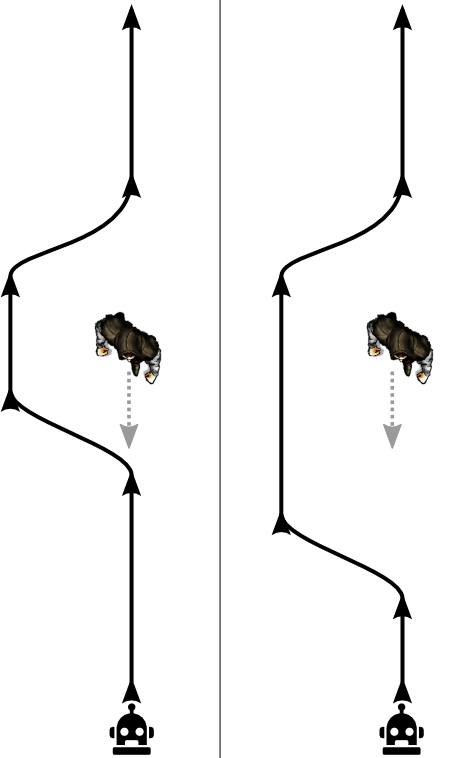
\includegraphics[scale=0.4]{figures/chapter2/condition_1_proactivity_shrink.png}
\caption{Influence of the modification of the TTC constraint cost weight on the trajectory. On the left, the weight is low, the robot will show the side and avoid the human at the last moment. On the right, the weight is high, the robot will show the chosen side and avoid the human much earlier.}
\label{ttc_explanations}
\end{figure}

Moreover, as stated before \unsure{maybe move the gaze stuff from related work to here?} several papers show that using the \textit{head} of a robot can significantly improve legibility and mutual manifestness. Thus, we also chose to make the robot look at its future planned trajectory as shown in Fig.~\ref{head_gaze_behavior}. This is possible thanks to the HATEB algorithm which, unlike many other local planner only publishing  speed commands \improvement{Adds ref to DWA for example ?}, also publishes a precise short-term trajectory. Finally, to show the robot awareness of the human presence, we made it \textit{glance} at the human twice when they enter a large and a small radius circle.

\begin{figure}[hbtp]
\centering
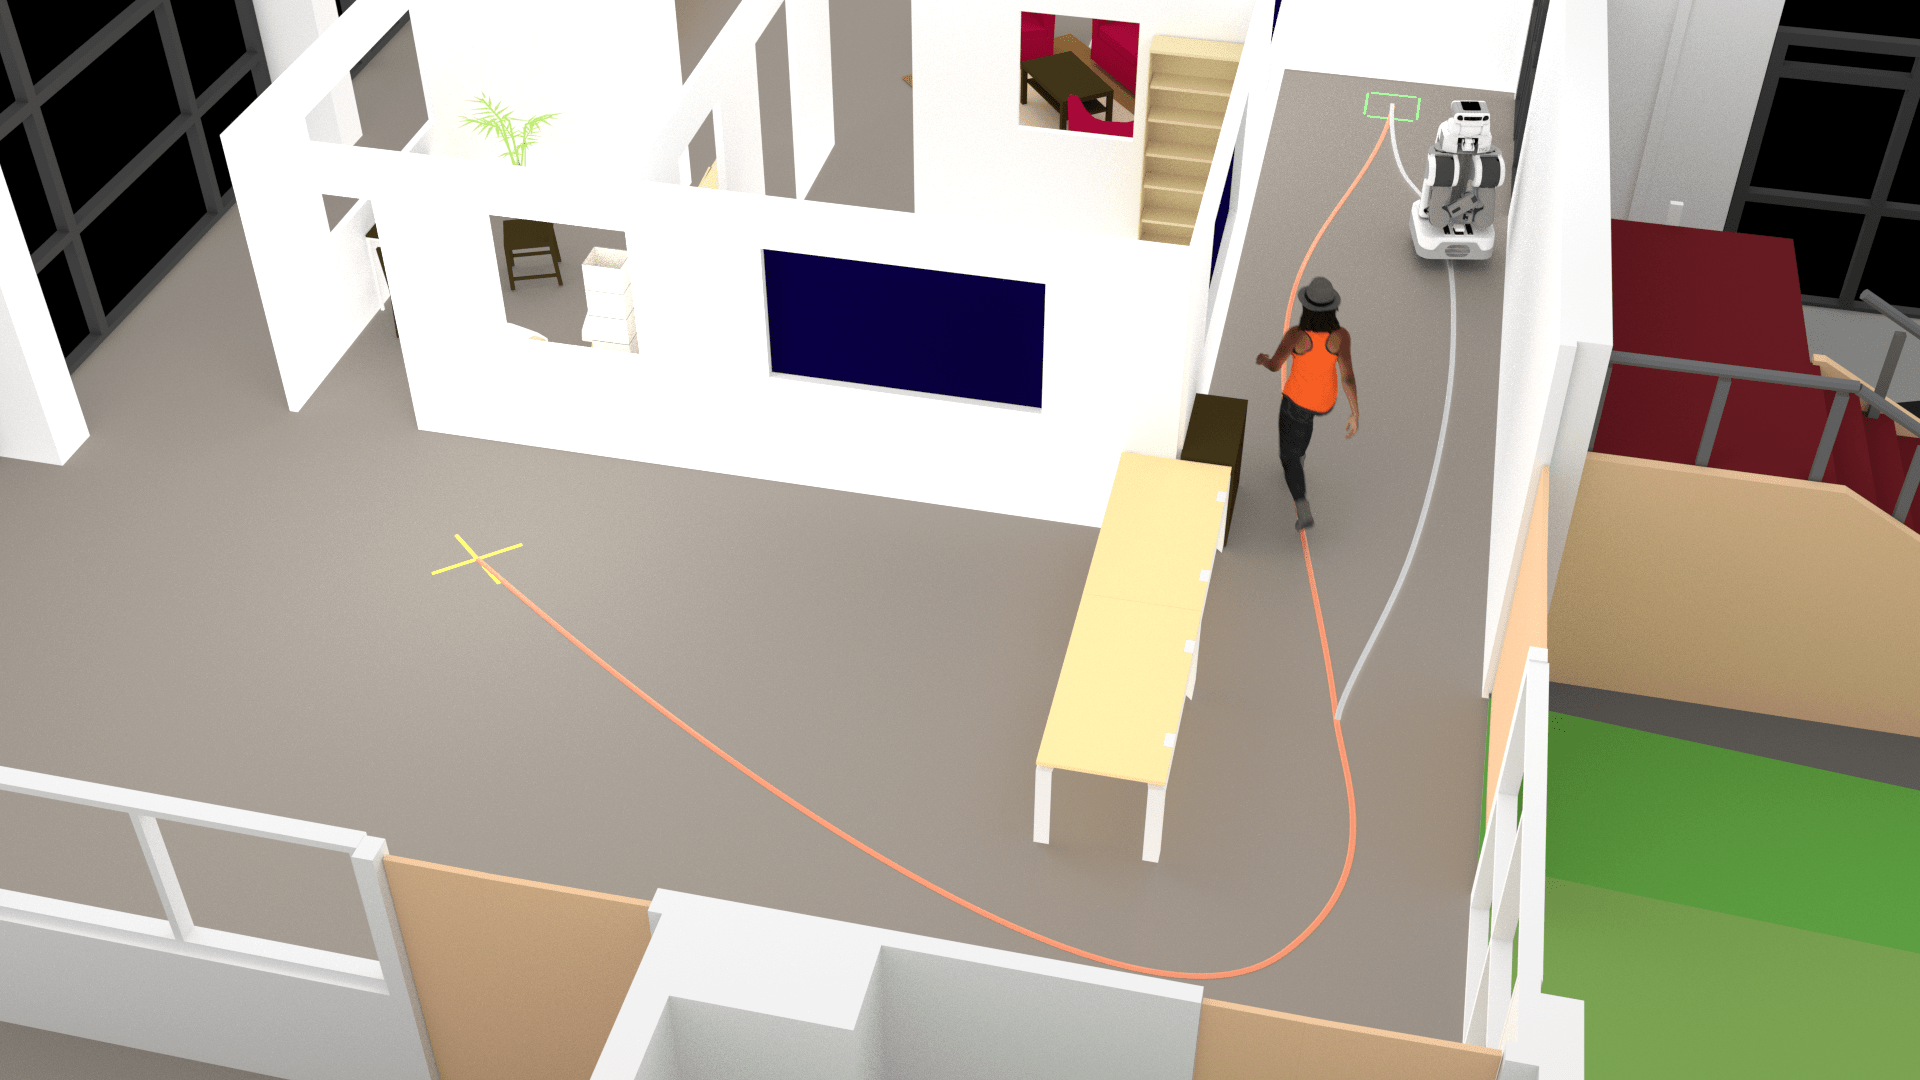
\includegraphics[scale=0.4]{figures/chapter2/expe_human-min.png}
\caption{Behavior implemented for the robot head. The robot \textit{looks} at a point placed at its planned position X seconds in the future and h meters above the ground.}
\label{experiment_adream}
\end{figure}

\subsection{User study protocol}

\begin{figure}[hbtp]
\centering
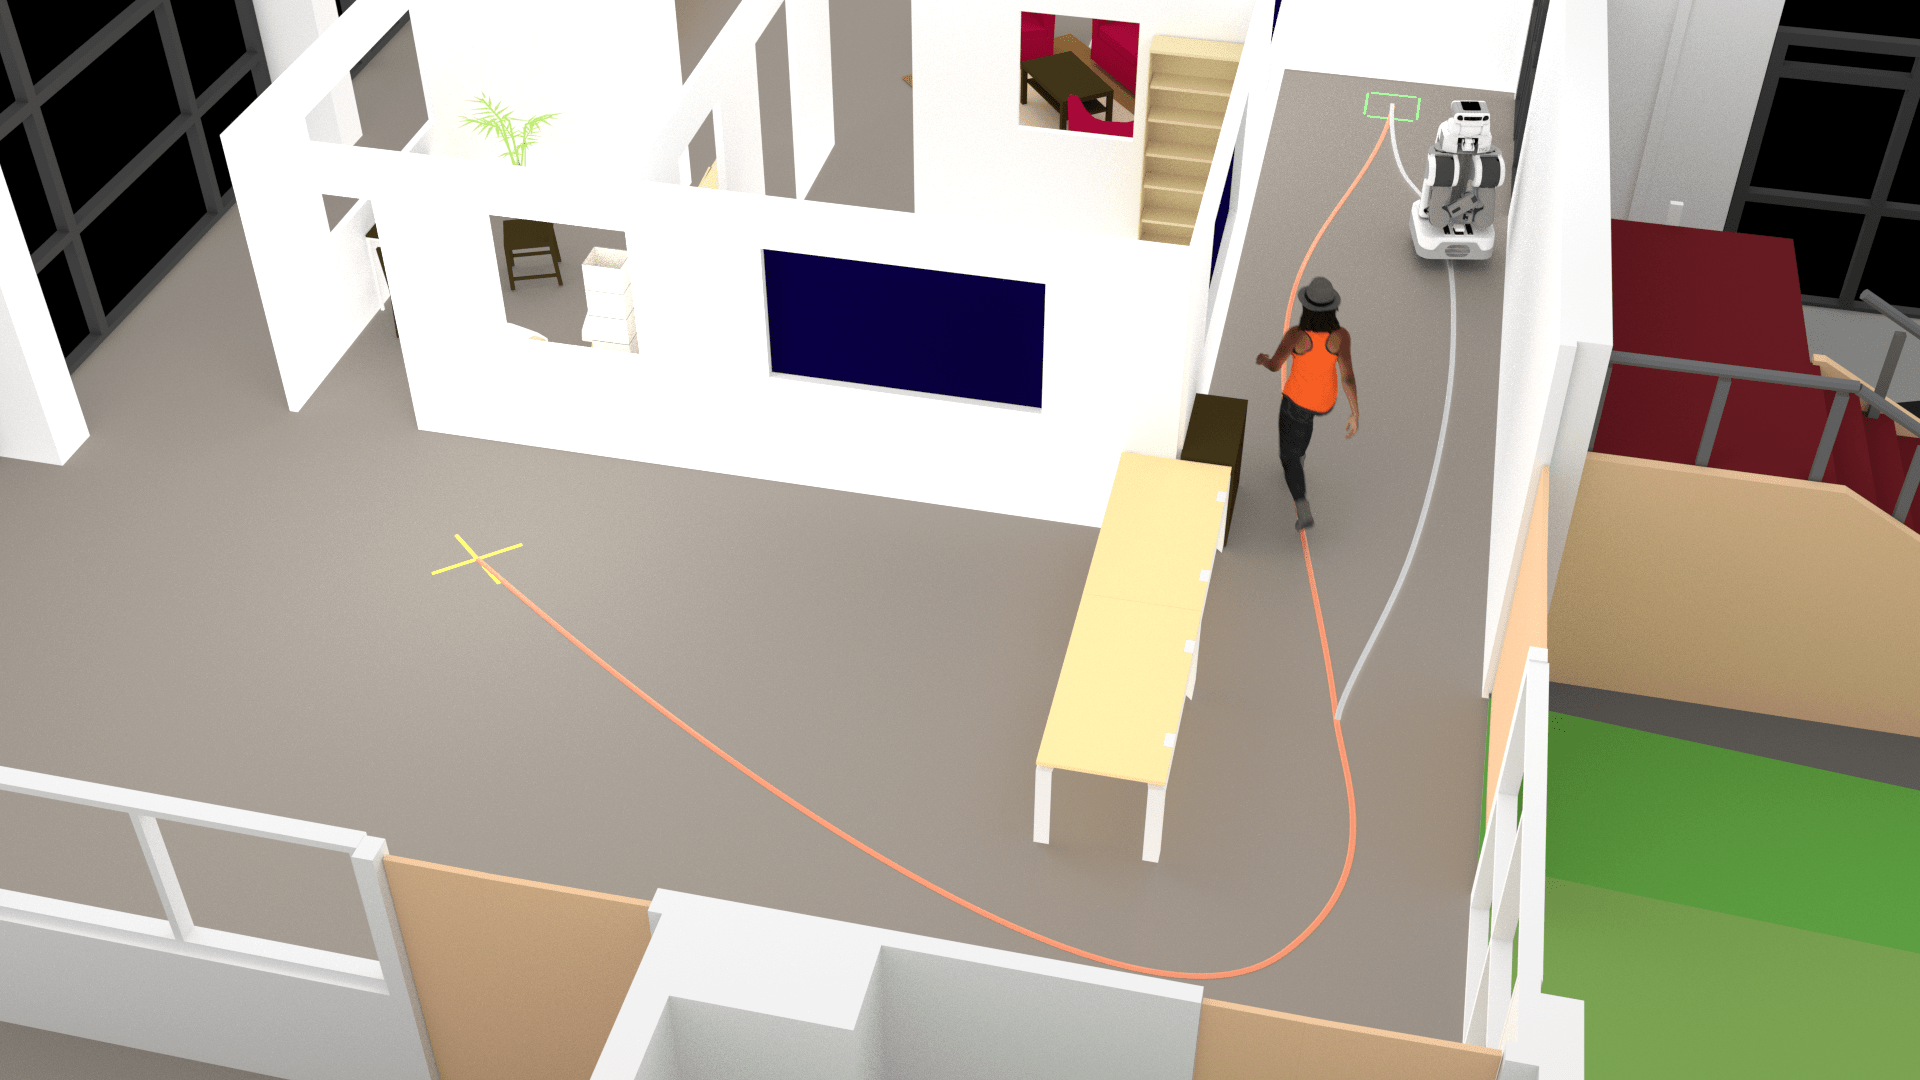
\includegraphics[scale=0.4]{figures/chapter2/expe_human-min.png}
\caption{The  study  environment.  The  participant  had  to  go  from  the  yellow  cross  marked  on  the  ground  to  the  green  square  also  marked  on  the  ground,which was the robot starting point. Crossing occurred roughly in the area where the robot and participant are on the picture. Trajectories are displayed on the picture for example only and where not marked on the ground or suggested by the experimenters at any time.}
\label{head_gaze_behavior}
\end{figure}

\subsubsection{Objective}
The aim of this study is to evaluate the impact of the TTC cost constraint and head behavior on usability. We designed an user study where actual individuals have to walk through a corridor facing a fully autonomous navigating robot. The afore-explained robot behavior was used. We measured the quality of the interaction between the robot and the human with both objective (visual behavior) and subjective data. The subjective evaluation was based on three dimensions: (1) perceived efficiency of the robot navigation, (2) user satisfaction and (3) situation awareness.

\subsubsection{Participants}
We recruited a total of 28 participants (12 males and 18 females) aging from 21 to 41 (mean: 27.32, SD: 4.13). All 28 participants had never used or interacted with a PR2 for navigation tasks, and had a neutral or good vision of robotics (mean: 5.96 over a 7 points Likert scale, SD: 1.07). This research complied with the tenets of Declaration of Helsinki. Informed consent was obtained from each participant.

\subsubsection{Material}
A Willow Garage PR2 robot, at its lower spine position was used in this experiment. The robot measured 1.33 meters from ground to top. The entire robot can be considered as anthropomorphic and possesses a two degrees of freedom head integrating cameras resembling eyes.

The participant position was tracked using an Optitrack motion capture system, tracking a worn solid headband. This system allowed the robot to track the human anywhere in the room, without looking at them.

The experiment was conducted in a L-shaped corridor (Fig.~\ref{experiment_adream}). The participant and the robot started from opposite side of the corridor. The participant had to walk 6 meters before entering the long straight corridor part and seeing the robot, then walk 13 meters.

We used a \textit{ETG 2w} eyetracker from SMI to collect the eye movement data of the participant. It is a portable device, allowing, after a short calibration process, to track the user gaze, and measuring where the user looks at. The data were analyzed using the \textit{BeGaze 3.6} software from SMI.

Three questionnaires and an interview were used to collect the subjective measures. \improvement{Add questionnaires in appendix}
\begin{itemize}
\item Pertinence of robot decision: The PeRDITA questionnaire \cite{devin_evaluating_2018}, jointly developed between the LAAS-CNRS and the CLLE in Toulouse, France, aims at evaluating the participant perceived pertinence of robot decision during a human robot collaborative task. In its complete form, it measures 5 dimensions: interaction, competence perception, verbal, acting and collaboration. However, in this study the robot is mute, and as the dimensions are independent we chose to remove the verbal dimension.
\item Situation Awareness: Several techniques exists to measure the situation awareness during a task \cite{endsley_design_1988}. However, they require to freeze and hide the situation to the user, and probe their working memory by questioning them about its near future. In our setup, we can't stop the robot and make it disappear while it is navigating. Thus, we have developed a series of 6 questions for measuring the user situation awareness. These questions are presented to the user just after the navigation, and ask them to rank on a 6 points Likert scale each 3 stages (2 questions per stage) of the Endsley's model: perception, comprehension and projection.
\item User satisfaction: For measuring the user satisfaction we used the AttrakDiff questionnaire. It is a standardized UX (User Experience) questionnaire measuring both hedonic qualities and global attractiveness. We used the french translation of this questionnaire \cite{lallemand_creation_2015}.
\item Interview: The interview was constituted of 8 semi directed questions always asked in the same order. These questions aimed at qualitatively evaluate the user experience, behavior and perception of the user during the navigation. The interviewer was only allowed to read the questions and to make the participant elaborate by asking neutral questions like \"why?\" or \"can you tell me more?\".
\end{itemize}


\subsubsection{Experimental design}
The user study was a 2 $\times$ 2 within-participants user study to evaluate how the time-to-collision constraint and the head behavior impact the robot navigation effectiveness efficiency and satisfaction. The independent variables were the HATEB time-to-collision cost parameters (both weight and threshold) and the head behavior. The conditions for the time-to-collision variable were $\gamma_ttc = 0.01$ (in Eq.~\ref{eq:hateb_obj_function}) with $\tau = 1s$ for the \textit{low TTC} condition and $\gamma_ttc = 15$ (in Eq.~\ref{eq:hateb_obj_function}) with $\tau = 4s$ for the \textit{high TTC} condition. For the both \textit{continuous} and \textit{alternated} head behavior conditions the robot head was pointing towards a the robot planned position in 1.5s in the future at 1m above the ground. In addition, in the \textit{alternated} head behavior, the robot pointed its head towards the human when they entered the long part of the corridor during 1.5s and again during 1.2s when the robot and human were 3.5m apart.
The participant goal position was marked with a square on the ground, and was the starting point of the robot. The robot final position was 10m straight ahead of its starting position. So, the participant was able to reach their natural walking speed before turning at the corner of the L shaped corridor. The robot was only started when the participant was about to turn (2m before the turn), giving the impression that the robot was coming from further away while ensuring that the crossing happened around the same place independently of the participant walking speed.

\subsubsection{Study procedure}
The evaluation was cut into 4 blocks. A block consisted in two same condition crossing followed by questionnaires filling. A crossing was composed by the placement of the participant and the robot on their respective starting positions, then the participant was free to go to their previously indicated goal location while crossing the robot. The three questionnaires were filled next to the participant starting location and were concerning only the two crossings made in the current block. The 4 conditions order were randomized between participants and the condition change was made between two block but never between the two crossings inside the same block.

Before starting the experiment trials, a training trial was made with the robot starting shifted to one side of the corridor and going in straight line with its head fixed looking straight. Just after this training trial, the participant was brought close to the robot and invited to inspect it. A specific head behavior was triggered making the robot head to follow the human allowing the participant to notice without being told that the robot was able to know their position and that its head could move. Moreover, the experimenter showed that robot arms were locked in place in a tucked position, and that they kept the emergency stop remote and was able to stop the robot at any time.

After the 4 blocks have been passed by the participant, the experimenter interviewed them. The audio was recorded and the answer written down.

The whole study lasted around 45 minutes per participant.

\subsubsection{Measures}
The analysis of the data was made on 27 participants because one did not fill all the questionnaires and their data were thus removed from the study. The quantitative data (questionnaires and oculometry) were analyzed using a non parametric two-way repeated measures Friedman ANOVA test.
\begin{enumerate}


\item \textit{Questionnaires}:
The three questionnaires have been passed 5 times each (one trial + four blocks). The results were codified from 1 to 7 for the PeRDITA, from 0 to 6 for the AttrakDiff and from 1 to 6 for the situation awareness questionnaire while taking care of reordering inverted items.

The PeRDITA Cronbach's alphas were for each dimension: $\alpha = 0.89$ for the interaction, $\alpha = 0.87$ for the competence, $\alpha = 0.85$ for the acting and $\alpha = 0.86$ for the collaboration.

For the situation assessment questionnaire, the Cronbach's alphas were: $\alpha = 0.93$ for the perception, $\alpha = 0.88$ for the comprehension and $\alpha = 0.87$ for the projection.

\item \textit{Oculometry}:
The oculometry data were split into two parts: before the robot crossing, and after the robot crossing (when the robot is behind the human). As we were not interested in where the participant gaze after the crossing occurred we did not analyze this part. The number and duration of fixations were measured for each of the 9 defined areas of interest (AOI) (Fig.~\ref{fig:aois}). The semantic gaze mapping method was used, it consists in manually selecting in which AOI each automatically detected fixation lays.

\begin{figure}[hbtp]
\centering
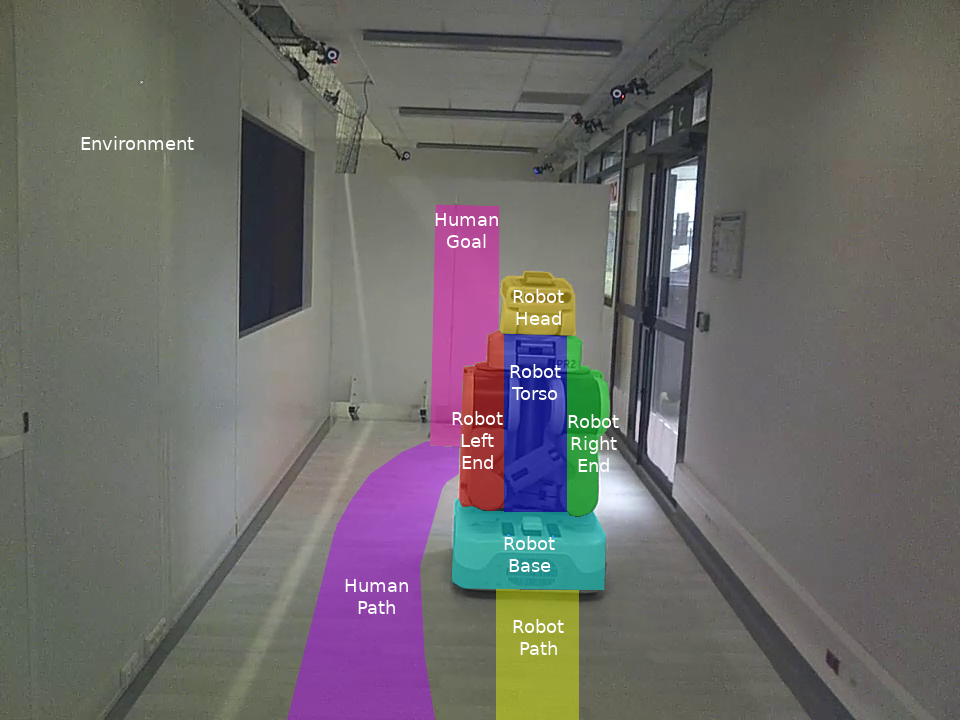
\includegraphics[scale=0.4]{figures/chapter2/pr2_aois_2.png}
\caption{The areas of interest defined to analyze the participants oculometric data.}
\label{fig:aois}
\end{figure}

\item \textit{Interview}:
The first question was a control question, ensuring that the participants saw differences between each blocks. After the second question, the interviewer revealed that the robot behavior was indeed different between each block, then proceeded to the rest of the interview. The participants answers were analyzed by excerpting verbatim (keywords or general ideas) from each question and computing their frequencies.

\item \textit{Dependent variables}:
Therefore, the dependent variables were the participant scores at the three questionnaires: PeRDITA, Situation Awareness and AttrakDiff, in addition to the number and duration of their gaze fixation during the crossing.
Prior to the experiment, the participants were asked to fill a questionnaire inquiring their age, gender, education level, profession, native language, an open question about past experience with robots and a 7 points Likert scale assessing their overall opinion about robotics.
\end{enumerate}

\subsection{Results}
\subsection{Quantitative results}
During the crossing almost all participants (95\%) went to their left (thus, letting the robot go to their right) because the experimental setup led them to do so as the interview revealed. The robot also planned that the optimal path (given the constraints described above) was to go to the right of the human. Participants who went to their right stated they were "testing" the robot, thus not respecting the given goal (which was to go to the marked goal and not to test the robot). These trials have been removed from the data.

\subsubsection{Pertinence of Robot Decision In joinT Action}
The mean scores of the three dimensions of the PeRDITA questionnaire were significantly higher with an alternating head behavior than with a continuous one. The quality of interaction was higher with an alternating head behavior (\textit{M} = 5.31, \textit{SD} = 0.97), than with a continuous head behavior (\textit{M} = 5.03, \textit{SD} = 1.17), \textit{F}(1,26) = 4.41, \textit{p} < .05, $\eta_{p}^{2}$ = .15. The perceived robot competence was higher with an alternating head behavior (\textit{M} = 5.12, \textit{SD} = 1.14), than with a continuous one (\textit{M} = 4.73, \textit{SD} = 1.14), \textit{F}(1,26) = 9.15, \textit{p} < .01, $\eta_{p}^{2}$ = .26. The quality of collaboration was higher with an alternating head behavior  (\textit{M} = 5.06, \textit{SD} = 1.04), than with a continuous one (\textit{M} = 4.73, \textit{SD} = 1.14), \textit{F}(1,26) = 6.07, \textit{p} < .05, $\eta_{p}^{2}$ = .19.

There was not any significant effect of TTC on the quality of interaction (\textit{F}(1,26) = 1.65, \textit{p} = .21.), on the perceived robot competence (\textit{F}(1,26) = 0.04, \textit{p} = .84), and on the quality of collaboration neither (\textit{F}(1,26) = 0.43, \textit{p} = .52). No interaction between TTC and head behaviors reached significance.

\subsubsection{Attrakdiff}
The mean score of the hedonic qualities dimension was higher with an alternating head behavior (\textit{M} = 5.06, \textit{SD} = 0.87), than with a continuous one (\textit{M} = 4.93, \textit{SD} = 0,82), \textit{F}(1,26) = 4.13, \textit{p} < .05, $\eta_{p}^{2}$ = .14. There was no significant differences regarding the scores of the pragmatic qualities (\textit{F}(1,26) = 0.34, \textit{p} = .57) and attractiveness (\textit{F}(1,26) = 0.14, \textit{p} = .71) dimensions. 

There was not any significant effect of TTC on hedonic qualities (\textit{F}(1,26) = 3.25, \textit{p} = .08), on pragmatic qualities (\textit{F}(1,26) = 2.97, \textit{p} = .10), and on attractiveness neither (\textit{F}(1,26) = 0.37, \textit{p} = .55). No interaction between TTC and head behaviors reached significance.

\subsubsection{Situation awareness}
The mean score of global situation awareness was significantly higher with an alternating head behavior (\textit{M} = 4.64, \textit{SD} = 0.98), than with a continuous one (\textit{M} = 4.33, \textit{SD} = 1.12), \textit{F}(1,26) = 7.77, \textit{p} < .01, $\eta_{p}^{2}$ = .23.

The mean scores of all the three dimensions of situation awareness were higher with an alternating head behavior than with a continuous one. Perception was significantly higher with an alternating head behavior (\textit{M} = 4.60, \textit{SD} = 1.08), than with a continuous one (\textit{M} = 4.15, SD = 1.29), \textit{F}(1,26) = 8.20, \textit{p} < .01, $\eta_{p}^{2}$ = .24. Comprehension was higher with an alternating head behavior (\textit{M} = 4.64, \textit{SD} = 1.05), than on a continuous one (\textit{M} = 4.36, \textit{SD} = 1.14), \textit{F}(1,26) = 5.99, \textit{p} < .05, $\eta_{p}^{2}$ = .19. Projection was higher (strong tendency) with an alternating head behavior (\textit{M} = 4.67, \textit{SD} = 0.96), than on a continuous one (\textit{M} = 4.47, \textit{SD} = 1.16), \textit{F}(1,26) = 3.52, \textit{p} = .07, $\eta_{p}^{2}$ = .12.

There was not any significant effect of the TTC on global situation awareness (\textit{F}(1,26) = 1.70, \textit{p} = .20), on the perception dimension (\textit{F}(1,26) = 0.72, p = .41), and on the comprehension dimension (\textit{F}(1,26) = 0.60, \textit{p} = .45). However, the mean score of the projection dimension was higher (strong tendency) with a high TTC (\textit{M} = 4.69, \textit{SD} = 0.98), than with a low TTC (\textit{M} = 4.44, \textit{SD} = 1.13), \textit{F}(1,26) = 4.03, \textit{p} = .06, $\eta_{p}^{2}$ = .13. No interaction between TTC and head behaviors reached significance.

\subsubsection{Gaze}
\begin{itemize}
\item  \textit{Robot vs. Environment}

The mean number of eye fixations was significantly higher on the robot (\textit{M} = 2.23, \textit{SD} = 0.98) than on the environment (\textit{M} = 1.17, \textit{SD} = 0.90), \textit{F}(1,21) = 17.82, \textit{p} < .001, $\eta_{p}^{2}$ = .46.
The mean number of eye fixations was higher (strong tendency) with a high TTC (\textit{M} = 1.76, \textit{SD} =  1.04) than with a low TTC (\textit{M} = 1.65, \textit{SD} = 1.11), \textit{F}(1,21) = 3.86, \textit{p} = .06, $\eta_{p}^{2}$ = .16, regardless of the AOIs. There was not any significant effect of the robot head behavior on the mean number of eye fixations, \textit{F}(1,21) = 0.90, \textit{p} = .35. No interaction between the three factors reached significance.

The mean average duration of eye fixations was significantly higher on the robot (\textit{M} = 351, \textit{SD} =  172) than on the environment (\textit{M} = 260, \textit{SD} = 123), \textit{F}(1,18) = 6.95, \textit{p} < .05, $\eta_{p}^{2}$ = .28. There was not any other significant effects or interactions regarding the average duration of eye fixations.

\item \textit{Robot AOIs}

As shown in Table~\ref{table:eye_fixation_ttc_head}, the head was the part of the robot that was the most fixated by the participants (\textit{M} = 6.13 ; \textit{SD} = 0.59), \textit{F}(4,84) = 39.10, \textit{p} < .001, $\eta_{p}^{2}$ = .65. The number of fixations on other parts were \textit{M} = 1.28 (\textit{SD} = 0.31) for the base, \textit{M} = 1.16 (\textit{SD} = 0.23) for the torso, \textit{M} = 0.95 (\textit{SD} = 0.19) for the right end, and \textit{M} = 1.64 (\textit{SD} = 0.37) for the left end. 

\begin{table}[!htbp]
   \caption{\label{table:eye_fixation_ttc_head} Mean number of eye fixations made by participants in each area of interest (AoI) of the robot in each experimental condition (TTC x robot head behavior) in main experiment. Standard deviations are shown in parentheses.}
    \begin{tabular}{lcccc}
    \hline
    \multirow{2}{*}{\textbf{Robot AoI}} & \multicolumn{2}{c}{\textbf{Low TTC}} & \multicolumn{2}{c}{\textbf{High TTC}} \\
    \cline{2-5} 
               & \textbf{Continuous}  & \textbf{Alternating}  & \textbf{Continuous}  & \textbf{Alternating}   \\
    \hline
    Head       & 5.64 (3.42)  & 5.50 (2.78)  & 5.93 (2.90)  & 7.45 (3.80)   \\
    Torso      & 1.39 (1.39)  & 1.14 (1.49)  & 1.39 (1.65)  & 0.73 (0.96)   \\
    Left end   & 0.95 (1.20)  & 1.07 (1.11)  & 1.00 (1.15)  & 0.77 (1.14)   \\
    Right end  & 1.82 (1.92)  & 1.55 (1.71)  & 1.55 (1.94)  & 1.64 (2.27)   \\
    Base       & 1.36 (2.07)  & 1.23 (1.53)  & 1.45 (1.65)  & 1.07 (1.27)   \\
    \hline
\end{tabular}
\end{table}

There was a significant interaction between the AOI type and the type of TTC, \textit{F}(4,84) = 5.72, \textit{p} < .001, $\eta_{p}^{2}$ = .21. The robot head was more fixated when the TTC was high (\textit{M} = 6.69, \textit{SD} = 3.43) than when it was low (\textit{M} = 5.57, \textit{SD} = 3.08). There was an interaction (strong tendency) between the AOI type and head behaviors, \textit{F}(4,84) = 2.34, \textit{p} = .06, $\eta_{p}^{2}$ = .10. The robot head was more fixated, when the robot head was alternating  (\textit{M} = 6.48, \textit{SD} = 3.43) than when it was continuous (\textit{M} = 5.78, \textit{SD} = 3.14).

In addition, there was a double interaction (strong tendency) between the AOI type, head behaviors and the type of TTC, \textit{F}(4,84) = 2.41, \textit{p} = .06, $\eta_{p}^{2}$ = .10. Table~\ref{table:eye_fixation_ttc_head} shows that the robot head was more fixated when the robot head was alternating only with a high TTC.

There was not any significant effect of the robot head behaviors on the mean number of eye fixations, \textit{F}(1,21) = 0.13, \textit{p} = .73. There was not any significant effect of the TTC type on the mean number of eye fixations, \textit{F}(1,21) = 1.82, \textit{p} = .19. The interaction between the TTC and the head behaviors, \textit{F}(1,21) = 0.74, \textit{p} = .40, did not reach significance.

The ANOVA for the mean duration of eye fixations was not possible due to an absence of data in some experimental conditions.
\end{itemize}

\subsection{Qualitative results}
All the participants saw differences between blocks, 19 of them saw head behavior differences and 10 of them saw trajectory differences. When the participant talked about the alternated head behavior, positive adjectives were employed ("reassuring", "sympathetic", "interactive"), when they talked about the continuous head behavior, negative adjectives were employed ("unsettling").

After the experimenter revealed that the robot behavior was different in each block, the participants preferred when the robot was "moving its head" (12 participants). Five participants also preferred when the robot changes its direction long before they cross. Participants did not appreciate when the robot kept a "fixed head" because they thought the robot was not aware of them (8 participants), when the robot was "hesitating" (4 participants) and when it came "too close" (4 participants).

Fourteen participants found the robot was the most competent in the condition with the alternated head behavior and high TTC, because the robot became aware of them when looking at them (10 participants), because the robot changed its direction sooner (4 participants), because it was trying to avoid them (4 participants) or because it was not coming too close (3 participants).

The participants found the robot more acceptable when it made a "visual contact" (4 participants) and when it changed its trajectory early (3 participants). They found the robot less acceptable when the robot came too close (6 participants), when hesitating (3 participants), when not making visual contact (2 participants).


\subsection{Discussion}
This study aimed at exploring how taking into account the human model and planning for both human and robot during navigation allows to easily design behavior enhancing the usability of the robot. More precisely, navigation coplanning allows to easily implement coordination smoothers and increase mutual manifestness, we thus hypothesized that these changes should lead to a significant impact on robot usability in the intricate scenario of narrow corridor crossing.

Human gaze analysis showed that head of the robot was fixed many times and even more when the robot showed its chosen corridor side early in the navigation (with a high TTC). Moreover, subjective results revealed that moving the head of the robot in an alternating pattern (pointing towards its path while sometimes pointing at the human head) improved the perception of the quality of interaction, the perceived robot competence, and the quality of collaboration. This alternative head behavior also increases the situation awareness score. This strongly support previous results on using the robot head during human robot navigation scenarios \cite{khambhaita_head-body_2016}, \cite{may_show_2015}.

However, the satisfaction seems to have been slightly improved (on hedonic quality) when the robot presented the alternating gaze behavior rather than the continuous one. This result is only a tendency, but in the interview, the participants identified as positive when the robot moved its head to glance at them and changed its trajectory. They also identified as negative when the robot was too close or did not look at them. We think these discrepancies between the AttrakDiff results and the interview are caused by our poor questionnaire choice. Indeed, the AttrakDiff questionnaire aims at measuring the satisfaction produced by a final product (\textit{e.g.} cellphones) and the willingness of a user to buy this product, but not the satisfaction of a user when dynamically interacting with a robot in a navigation scenario. Yet, as no other questionnaire to our knowledge proposed to measure user satisfaction during human robot interaction, we chose the AttrakDiff.

Results show that using the HATEB navigation co-planner with a high time-to-collision weight constraint cost and low threshold, alongside an head behavior signaling future robot trajectory and the human awareness during a crossing in a constrained space allows the human to have a better situation awareness and to perceive the robot as acting more pertinently and being more competent. This finding support the result from Lu et al. \cite{lu_towards_2013}, where the navigation efficiency is increased when the robot looks at the human and shows a "social" navigation behavior.

We speculate that both the high TTC and alternating gaze of the robot are needed to improve the interaction and that no simple effect are significant for multiple reasons. First, with only the robot choosing a corridor side early in the crossing (high TTC condition) without showing the human awareness (continuous head condition), it may not be obvious to the human that the trajectory change is due to their presence. Conversely, when the robot signals its awareness of the human (here by pointing its head towards them) but without taking any action to ease the interaction (low TTC condition), the human stays in a situation where they don't know what the robot will do next. Finally, by both making the robot show its human awareness and change its own trajectory to facilitate the interaction (coordination smoother), it becomes clear the that robot is proposing a co-navigation solution where both agents are avoiding each other.

Finally, oculometry results indicate that when the head is recognized as an information provider (in the alternating head condition), information are most likely to be sought in the robot head motion. The head is also looked longer when the robot alternately looks at the human. We can also note that people tend to think PR2 is getting data through its head, probably because of the visible cameras on it, even when it is not the case (like in our experiment).

\improvement{Ajouter limites et future works de l'étude ? Ou le mettre dans la section conclusion ?}

\section{Extending HATEB}
Having shown that providing co-navigation solution using HATEB can effectively be used to enhance the efficiency of the interaction, we will present in this section the different extensions made to HATEB.

\subsection{Adapting HATEB to other robots}
Khambhaita et al. \cite{khambhaita_head-body_2016} successfully used HATEB on a PR2 robot, both in simulation and on the real platform. As the approach is general, we implemented it on other robots.

\subsubsection{Humanoid Robot}
Humanoid robots are characterized by their bipedal navigation, tremendously increasing the complexity of simple navigation with regards to wheeled robots. However, legged robots present a large advantage for social and human robot interaction as human infrastructure are often thought for being navigated with legs rather than with wheels. Thus, we tried to implement our approach to a humanoid robot.

To do so, we partnered with the Gepetto team at LAAS-CNRS specialized in humanoid systems motion. Thanks to their modular software architecture presented in \cite{stasse_modular_architecture_2008}, only minor changes had to be done to HATEB to integrate with their other components.

One of their component \cite{naveau_reactive_walking_2017} takes as parameter a (simplified) robot kinematic model and is able, in real-time and at typical joint position control frequencies (around 200~Hz), to give position command to all the robot joints in order for the center of mass of the robot to respect a speed command given as input. To do so, the component needs to generate footstep placements and to compute robot joint positions ensuring the equilibrium and the respect of the kinodynamic constraints (between two successive poses) of the robot. However, this component as no ROS interface whereas HATEB is heavily built for ROS use. Thus, we made a bridge transferring the speed commands output by HATEB to the Gepetto architecture and transferring back the joint position commands.

This has only be run virtually, and for simplicity, no simulator was used. Instead, we assumed the joint position command to be immediately and perfectly executed. Such an assumption has been made possible because of the effectiveness of the Gepetto architecture, having a tested precise model of the robot, ensures that the kinodynamic constraints will be respected, and consequently gives a correct robot behavior.

We tested this approach on a virtual HRP2 robot, with a virtual human. \unsure{What result do I have from that?} 

\subsubsection{Pepper robot for close human robot motions}
The European project MuMMER aimed at deploying a Pepper robot in a shopping mall in Finland to entertain and guide customers. \improvement[inline]{ref} The project united seven different stakeholders bringing their knowledge to the project. The LAAS-CNRS goal was to make the guide task. However, in order to serve the most customers possible and to cope with large navigation issues of the Pepper platform, we choose not to go with the customer all the way to the asked shop, but instead, as the mall employees usually do, give directions to the customer to help them find the requested shop.
However, giving only verbal instructions concerning the route is not sufficient, we chose to make the robot point the shop, if it is visible from the current position, or point its direction and the first visible element of the route otherwise.

Although, the surroundings of the robot home place (the place in the mall where the robot is located, and thus, where the interaction takes place) contains some obstacles such as barriers, structure poles and advertisement posters. Thus, the object the robot has to point to the human might not be visible from their current position. We thus endowed the robot with the ability to compute the optimal position for the human and the robot for it to point at a landmark. This computation details can be found in \cite{waldhart_reasoning_shared_2019}. Once the robot has computed these optimal positions, it needs to move to its one while ensuring the human can move to theirs. Moreover, the customers might be hesitant to approach the robot to start an interaction, thus, the robot is also able to approach a nearby human to ask them if they need its help. However, it has to consider that the human might also move towards the robot to encounter it.

To tackle both of these issues, we decided to use HATEB. We made a higher level component proposing three services: rotate, navigate to and approach. While the rotate service is only made for in place rotation of the robot in order to reorient itself for repositioning or to look or point at something, the other two uses the HATEB planner described earlier. The navigate to service expects a robot goal pose and optionally a human identifier and a human goal (which is shown by the robot before starting the navigation). The HATEB planner is then called with empirically tuned weights to make the robot navigate to its goal position while, if provided, ensuring the human can reach theirs. The approach service expects a human identifier and a distance, and use the HATEB planner with different weights (e.g. with the visibility constraint described in \ref{sec:visibility_constraint} activated) with a goal at the specified distance in front of the human. The human goal is predicted from their current pose and velocity some seconds in the future, and updated at each control loop with their new sensed pose and speed.

While this scheme worked well for the approach, with the robot presenting an efficient approach trajectory reacting the human motion, it performed very poorly for the navigation part. Indeed, the robot navigation was erratic and made too long trajectories even between close start and goal points. We identified two causes to this over conservative behavior:

\begin{itemize}
\item First, the HATEB algorithm did not support holonomic motion. Although this was not a problem for long distance scenarios, it made the robot having to maneuver to achieve small displacements.

\item Then, by planning these short trajectories so close to the human, the optimizer does not have a lot of latitude to play with, and the search space is very noisy and chaotic.
\end{itemize}

It has thus been decided in the project to not use the HATEB approach, but simply an holonomic timed elastic band enriched with social constraints linked to the nearby humans (\textit{i.e.} only optimizing the robot trajectory and not the human one).

This allowed to point out some of the limitations of the HATEB approach, it performs poorly for small, intricate displacements. This led to the creation of HATEB2 \cite{teja_hateb2_2020}, which is able to switch online between the HATEB planner, the TEB planner with social constraints or a velocity obstacle planner.

\unsure{HATEB 3D ?}

\subsection{Using the estimated time to goal to measure the execution of the planned trajectory}

Another benefit of the HATEB approach is that it does not only compute speed command to follow a global plan while avoiding obstacles like other classic local planner, but also returns a complete short term trajectory for both the robot and the human. Moreover, as the trajectories contains the expected duration between each pose, simply by summing them, we can have an estimate of the time remaining to execute the local trajectories. Besides, we also compute the estimated time remaining for the global trajectories after the local ones by dividing the computed speed at the last local trajectory pose by its length. By summing these two estimated remaining times, we can have a estimation of the remaining navigation time (the time to goals) for all the considered agents.

By monitoring the evolution of these times, we can estimate a quality of the ongoing navigation. Indeed, the local trajectories are computed at at a position control rate and so are the time to goals. Intuitively, if the computed time to goals are decreasing at the same rate as the real time duration (\textit{e.g.} the estimation for the robot goes from 12 seconds to 11 seconds while one second has elapsed) the execution of the trajectories are going according to plan. Instead, if the computed time to goals are decreasing slower than the real time duration, staying equals or even increasing, the execution does not go as smoothly as the plan was.

We formalized it as follows: 
\begin{equation}
s_i(t) = \frac{ttg_i(t) - ttg_i(t - x)}{x}
\end{equation}
with $s_i(t)$ is the time to goal variation for the trajectory $i$ (either the robot or one of the considered human) at time $t$, and $x$ is the time window size parameter, specifying how old are the previous time to goal value we are comparing the current one with.
With this definition we have:
\begin{itemize}
\item $s(t) \approx 1$: the execution goes according to plan,
\item $s(t) > 1$: the execution outperforms the plan,
\item $0 < s(t) < 1$: the execution goes slower than the plan, but progress towards the goal is still being made,
\item and $s(t) < 0$: the goal is getting further.
\end{itemize}

This value can then be fed back to a supervision system which can change the navigation parameters or abort it to make a repair strategy if, combined with other task monitored values, it judges the navigation action is endangering the higher level task.

\improvement{Dire que même si ça permet une certaine évaluation ça ne dit pas le problème. Obstacle imprévu par le robot ? Human qui change d'avis ? Humain qui ne veut pas coopérer ? Mauvais modèle de l'humain ?}



\subsection{Adding constraints}
\unsure{Is this subsection useful ?}

\subsubsection{The visibility constraint}

\unsure{ttc plus ?}


\section{Conclusion}

\ifdefined\included
\else
\bibliographystyle{acm}
\bibliography{These}
\end{document}
\fi
